% Typeset with XeTeX
% Allows use of system fonts rather than just LaTeX's ones
% NOTE - if you use TeXShop and Bibdesk (Mac), can complete citations
%  - open your .bib file, type~\citep{xx... and then F5 or Option-Escape
\documentclass[11pt]{article}
\usepackage[margin=1in, letterpaper]{geometry} % set page layout
%\geometry{letterpaper}  % or a4paper
\usepackage[xetex]{graphicx} % allows us to manipulate graphics.
% Replace option [] with pdftex if you don't use Xe(La)TeX
\usepackage{color}
\usepackage{indentfirst}
\usepackage{hyphenat}
\usepackage{epstopdf} % automatic conversion of eps to pdf 
\usepackage{amsmath, amssymb} % Better maths support & more symbols
\usepackage{textcomp} % provide lots of new symbols - see textcomp.pdf
% line spacing: \doublespacing, \onehalfspacing, \singlespacing
\usepackage{setspace}
\singlespacing
\usepackage{pgfplotstable}
% allows text flowing around figs
% use \begin{wrapfigure}{x}{width} where x = r(ight) or l(eft)
\usepackage{wrapfig}
\usepackage[parfill]{parskip} % don't indent new paragraphs
\usepackage{flafter}  % Don't place figs & tables before their definition 
\usepackage{verbatim} % allows \begin and \end{comment} regions
\usepackage{booktabs} % makes tables look good
\usepackage{bm}  % Define \bm{} to use bold math fonts
% linenumbers in L margin, start & end with \linenumbers \nolinenumbers,
\usepackage{lineno} % use option [modulo] for steps of 5
\usepackage[auth-sc]{authblk} % authors & institutions - see authblk.pdf
%\renewcommand\Authands{ and } % separates the last 2 authors in the list
% control how captions look; here, use small font and indent both margins by 20pt
\usepackage[small]{caption} 
\setlength{\captionmargin}{20pt}

%: FONT
% If you don't want to use system fonts, replace from here to 'Citation style' with \usepackage{Palatino} or similar
%: ************ FANCY FONTS START HERE
\usepackage[no-math]{fontspec} % 'no-math' = keep computer modern for math fonts
\usepackage{xunicode} % needed by XeTeX for handling all the system fonts nicely
\usepackage[no-sscript]{xltxtra} 
\setmonofont[Scale=0.8]{PT Serif} % typeface for \tt commands
\setsansfont[BoldFont={PT Serif Bold}, ItalicFont={PT Serif Italic}]{PT Serif} 
\defaultfontfeatures{Mapping=tex-text}
\setmainfont{Minion Pro}
%\setmainfont{Source Sans Pro}

%: ************ FANCY FONTS END HERE

%:CITATION STYLE
% natbib package: square,curly, angle(brackets)
% colon (default), comma (to separate multiple citations)
% authoryear (default),numbers (citations style)
% super (for superscripted numerical citations, as in Nature)
% sort (orders multiple cites into order of appearance in ref list, or year if authoryear)
% sort&compress: as sort, + multiple citations compressed (as 3-6, 15)
\usepackage[numbers,comma,sort&compress]{natbib}

%:SHORTCUT COMMANDS
% Maths
\newcommand{\ddt}[1]{\ensuremath{\frac{{\rm d}#1}{{\rm d}t}}}  % d/dt
\newcommand{\dd}[2]{\ensuremath{\frac{{\rm d}#1}{{\rm d}#2}}} % dy by dx  - \dd{y}{x}
\newcommand{\ddsq}[2]{\ensuremath{\frac{{\rm d}^2#1}{{\rm d}#2^2}}} % second deriv
\newcommand{\pp}[2]{\ensuremath{\frac{\partial #1}{\partial #2}}} % partial \pp{y}{x}
\newcommand{\ppsq}[2]{\ensuremath{\frac{\partial^2 #1}{\partial {#2}^2}}}
\newcommand{\superscript}[1]{\ensuremath{^{\textrm{#1}}}} %normal (non-math) font for super/subscripts in text
\newcommand{\subscript}[1]{\ensuremath{_{\textrm{#1}}}}
\newcommand{\positive}{\ensuremath{^+}}
\newcommand{\negative}{\ensuremath{^-}}
% Editing
\newcommand{\red}[1]{{\color{red}{#1}}}
\newcommand{\redtext}[1]{{\color{red}{#1}}}
\newcommand{\blue}[1]{{\color{blue}{#1}}}
\newcommand{\bluetext}[1]{{\color{blue}{#1}}}
\newcommand{\scinot}[2]{\ensuremath{#1 \times 10^{#2}}}
% Standard stuff
\newcommand{\be}{\begin{equation}}
\newcommand{\ee}{\end{equation}}
\newcommand{\bea}{\begin{eqnarray}}
\newcommand{\eea}{\end{eqnarray}}
\newcommand{\ie}{\textit{i.e.}}
\newcommand{\etal}{\textit{et al.}}
\newcommand{\khi}{Ki67$^\text{hi}$}
\newcommand{\klo}{Ki67$^\text{lo}$}


% \begin{graybox} text \end{graybox} for text with a background colour
\definecolor{MyGray}{rgb}{0.96,0.97,0.98}
\definecolor{MyGray}{rgb}{0.96,0.90,0.98}
\makeatletter\newenvironment{graybox}{%
	\begin{lrbox}
	{\@tempboxa}\begin{minipage}[r]{0.98\columnwidth}}{\end{minipage}\end{lrbox}%
	\colorbox{MyGray}{\usebox{\@tempboxa}}
}\makeatother


%%%%%%%%%%%%%%%%%%%%%%%

\title{Population dynamics of  B cell subsets -- analysis and predictions}
\author{}

\date{}

\begin{document} 
\maketitle

We aimed to quantify the dynamics of various subsets within mature B cell population and to understand the rules of replacement of old cells by that of new ones within each subset.  We adopted the conventional view of B cell development and assumed that Transitional 2 (T2) cells are the direct precursor of FM cells, which then participate in germinal centre (GC) reactions upon antigen interaction. We also assumed that both FM and T2 cells circulate freely in the lymphatic system, and so we pooled the numbers of these subsets in spleen and the lymph nodes when modelling their dynamics.

%We define turnover to mean loss. 

% In the busulfan chimeras, if the source is constant in time and all cells behave the same way, the existing population is replaced at rate $\lambda$, the net loss rate (turnover rate - division rate). 

%So rate of replacement is not necessarily the rate of turnover (unless there is no division). Division compensates for turnover and keeps host cells in the pool for longer.

%Might be worth coming up with a word for $\lambda$. I think 'clonal persistence --- low $\lambda$ means that a cell and its progeny survive for a long time (if $\lambda=0$, a clone persists for ever even though it may be dividing and dying; if $\lambda>0$, mean lifetime of a lineage (e.g. a cell and all its descendents) is $1/\lambda$. If $\lambda>0$, the cell population grows exponentially as $e^{\lambda t}$. 


%\red{One concern: Sanket tried T1 as source and it actually gives better fits in all FM cases ($\Delta$AIC $\simeq$ 5). But we are going with dogma and saying T2 is source. It's puzzling to us that there is apparently so much residual Ki67 expression in FM from the T2 source, if all the division is pre-T1 as you say. Makes me worry a littl...} 

\section*{Follicular Mature B cells}
\subsection*{Replacement kinetics are consistent with FM cells being a single, kinetically homogeneous population, with cell lifetime increasing with host age}
The normalised donor fraction $f_{d}$ in the FM compartment stabilises close to 1 by about 120d post-BMT, implying the near-complete replacement of the compartment within that timeframe. Complete replacement suggests that the average rates of loss across host and donor cell populations are always equal.
We modelled this behaviour by assuming that cells differentiate into FM B cells at a rate proportional to numbers of T2 cells, and all FM cells, whether host or donor, are lost through death or differentiation  at rate $\delta$ and renewed through division  at rate $\rho$. For generality we allowed either of these rates to vary with the age of the host. We fitted each model  simultaneously to the timecourses of the total size and donor cell chimerism of the FM population (Figure~\ref{fig:results_FM}A and B; see Methods for details). We found strongest support for a model in which the loss or turnover rate $\delta$ changes with host age and the division rate $\rho$ remains constant. Specifically, total numbers of FM B cells are given by
\be
\ddt{N_\text{FM}} = \;  \phi(t) + (\rho - \delta_{0}e^{-rt}) N_\text{FM},
\label{eq:FM_total}
\ee
where $\phi(t)$ is the daily rate of influx from T2, which changes little with host age but whose timecourse was estimated using a (nearly flat) spline, and time is measured from age 40 days, at which time the loss rate is $\delta_{0}$. This model was superior to the simplest model with constant rates of division and turnover ($\Delta$AIC = 5.9) and also superior to the alternative with a time-varying division rate ($\Delta$AIC = 12). We estimate that FM B cells divide slowly, on average every 56 days,  and have a mean residence time (lifetime) of 18 days in 40 day-old mice. This life expectancy doubles approximately every 14 months. We also predict that approximately 4\% of FM B cells are replaced each day by newly differentiated cells from the T2 population. Parameter estimates and 95\% confidence intervals are in Table 2.
\red{We also define the net loss rate $\lambda$ as the aggregate of cell division and turnover (i.e. $\delta - \rho$), which decreases with time for FM cells, as $\delta$ declines.
	Therefore, in old animals individual FM clones and their progeny would persist longer in follicles than in younger animals, purely due to age-mediated changes in the host environment.}

%Even with the low levels of proliferation seen in FM cells longer-lived clones are possible because of increase in survival rate of cells and their progeny.

\subsection*{No evidence for  heterogeneity or cell-age dependent effects within FM B cells}

The decline we detect in $\lambda$ with host age, which we infer derives from progressively increased survival within the FM compartment, therefore drives  a gradual slowing of the approach to stable chimerism relative to the kinetic predicted by a simple model of constant division and turnover. An alternative explanation of this time-varying kinetic is that the FM pool comprises independent sub-populations with different but constant rates of division and turnover, each fed from the T2 source.  In this scenario, less persistent populations (those with a high net loss rate $\lambda$) will be replaced most rapidly after BMT, giving an initial steep upslope in chimerism. There will then follow a slower increase as the more persistent FM subpopulations (with low $\lambda$) are replaced by donor cells relatively slowly.

We fitted a model of kinetic heterogeneity assuming two independent subpopulations, allowing their relative size and their constant loss rates $\lambda_{1}$ and $\lambda_{2}$ to be free parameters. However this model received lower support than the model of FM cells as a single population with turnover slowing with host age ($\Delta$AIC = 12, Table \ref{tab:FM-AICs}).   Indeed there was a very weak signature of kinetic heterogeneity;  the estimated net loss rates of the two FM subpopulations  were nearly equal  ($\lambda_{1} =\delta_{1} -\rho_{1}$ = 0.039 (0.025, 0.062) and  $\lambda_{2}$ = 0.028 (0.023,0.033)) and close to that of the simplest homogeneous model with $\lambda$ = 0.029 (0.024, 0.033).

We also found no evidence for any host-donor differences in kinetics in the form of a persistent host-derived `incumbent' population, or any change in the net rate of loss of loss with cell, rather than host, age (Table~1). For a discussion of these models, see Hogan et al. PNAS 2015 and Rane et al. PLoS Biology 2018 (in press)). 

Another potential mechanism for slowing replacement with host age is a decline in the rate of influx (e.g. a fall in the rate of differentiation from T2) with host age. We found no evidence for this ($\Delta$AIC > 10), and were close to overfitting at this point.

\begin{figure}[h!]
	\centerline{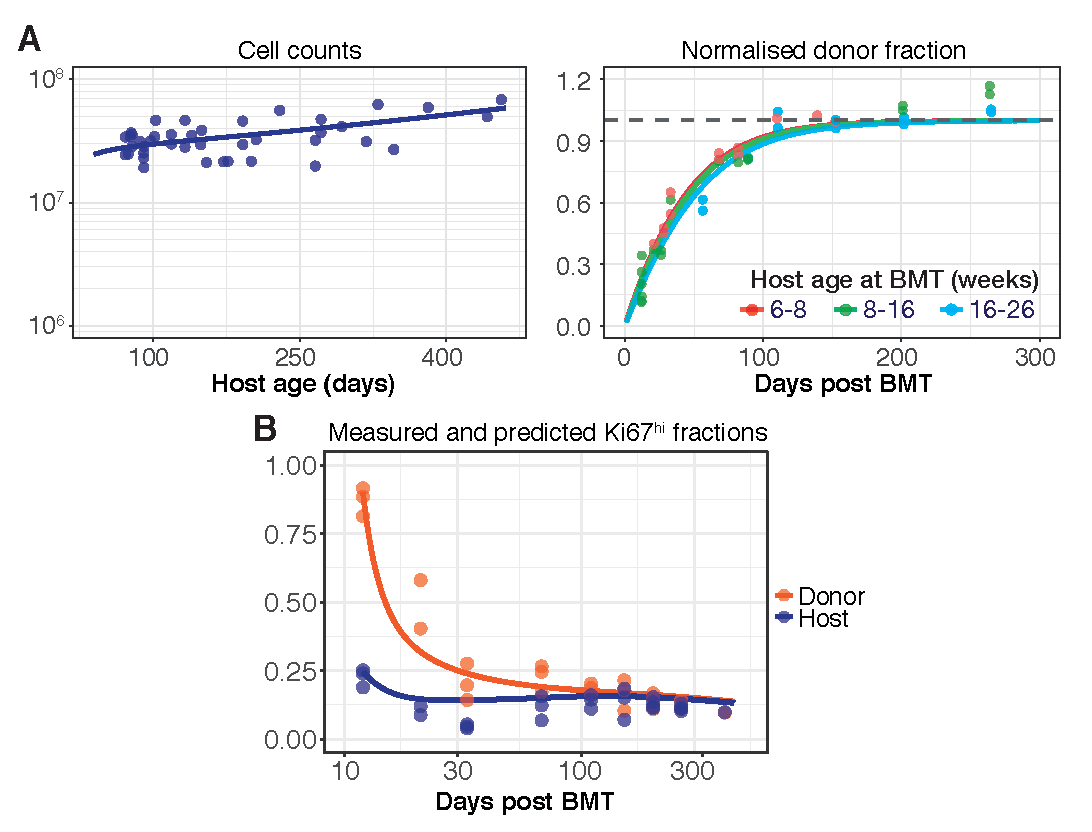
\includegraphics[scale = 0.85] {Results_FM.pdf}}
	\caption{\small \textbf{Fitted and predicted   population dynamics of FM B cells, using the best-fitting model in which cells divide at a constant rate and their mean residence time increases with host age.}  (A) The model was fitted simultaneously to the extended timecourses of total cell counts of FM B cells pooled from LN and spleen in busulfan chimeras,  and the donor fractions in FM B cells normalised to the chimerism in T2 cells. The latter took account of different ages at BMT (right-hand panel, coloured lines; each generated using the  mode of the age within each group). (C) We then used the model parameters to predict the proportion of cells that were \khi\ within host and donor FM B cells over time.}
	\label{fig:results_FM}
\end{figure}

\subsection*{The model of time-varying loss successfully predicts the kinetics of Ki67 expression within host and donor populations}
As well as the numbers of host and donor-derived cells in the FM compartment, we  also measured the kinetics of their expression of Ki67, a nuclear protein expressed during cell cycle and lost with a lifetime of 3-4 days following mitosis (Gossel eLife 2017 \red{and others - see refs in that paper}). Immediately following BMT the donor FM cells are highly enriched for recently divided cells, with around 80\% \khi, but this proportion falls slowly to equalise with that of host cells at around 10\% after approximately 100 days (Figure~\ref{fig:results_FM}C, red and green points).

As a validation of the models,  which were fitted only to the timecourses of total FM B cell numbers and chimerism, we used them to predict the dynamics of Ki67 expression within host and donor cells over time. The best-fitting time-dependent homogeneous model  predicted these kinetics remarkably well. These predictions were generated by inserting the estimated rates of loss ($\delta(t) = \delta_{0} e^{-rt}$) and division ($\rho$) into a model which explicitly follows the transit of cells between \khi\ and \klo\ states, which we have employed previously (Hogan PNAS 2015, Gossel eLife 2017). We assumed a mean lifetime of Ki67 post-mitosis of 3.5d, and also assumed that \khi\ and \klo\ cells are lost at equal rates $\delta(t)$. The timecourses of host and donor \khi\ fractions were then generated by simulating the model with its best-fit parameters, beginning at the mean \khi\ fractions observed at 12d post-BMT, pooled across all experimental cohorts. See Methods below for details.

The simulations show that the host/donor disparity in Ki67 expression derives largely from residual expression of Ki67 on cells that have recently entered the FM pool from the T2 precursor population \red{T2s are not dividing, you say... so surely this is further evidence that T1s are the source for FMs?}.  Soon after BMT, the donor FM pool is highly enriched for these recent immigrants, roughly 80\% of which are Ki67,  relative to the more established host-derived pool. The lifetime of FM cells is relatively short and so a substantial fraction of newly immigrated \khi\ cells  are lost before they transition to \klo. This interplay means that quiescent donor cells are slow to accumulate. In parallel, Ki67 levels transiently dip in host FM cells following BMT due to the sudden reduction in influx from the host T2 pool, before they re-establish equilibrium at lower numbers. 

\subsection*{Summary}
\begin{itemize}
\item Most support for model in which FM B cell residence time increases with host age
\item No evidence for kinetic heterogeneity (\ie\ multiple subpopulations with different turnover, or host incumbents) 
\item No evidence for changes in the per-cell rate of differentiation from T2 with cell age
\item No evidence for changes in rates of loss or division of FM cells with cell age.
\end{itemize}

%of \khi\ fractions within host and donor compartments .
%The possible explanation for this is that majority of ki67 in FM compartment is source derived suggesting that FM cells are primarily maintained by high influx from source and by very low levels of cell division.
%The high influx corresponds to high loss rate (inverse of residence time, Table~\ref{tab:FM-parestm}) in the FM subset, which only allows for slow accumulation of \klo\ cells post BMT in the donor compartment. 
%Inflow of very high (> 90\% of donor influx) numbers of \khi\ cells with gradual accrual of \klo\ population, temporarily maintains high fractions of \khi\ cells within donor compartment, which slowly stabilise to levels equivalent to that of the host compartment as donor fractions stabilise.
%In the host compartment, since pre-existing cells are mostly \klo, the low inflow ($\chi \sim$ 0.8)  of new \khi\ cells doesnt alter the kinetics of \khi\ fractions within these cells.
%In summary, we find no strong evidence for heterogeneity within FM B cells which are suggested to be firmly regulated by the homeostatic factors changing with the age of the host.


%: Table 1
\begin{table}[h!]
	\begin{center}
		\renewcommand{\arraystretch}{1.25}
		\begin{tabular}{c c c c c} 
			\toprule 
			 \multicolumn{5}{c}{\textbf{Model and $\Delta$AIC}} \\
			\cline{1-5}
			 {\small Time-dependent}  & {\small Simple homogeneous} &  {\small Kinetic heterogeneity} & {\small Incumbent}  & {\small Age-structured} \\ 
			\toprule
			 0      &  5.9  & 12 & 12  &  12  \\ 
			\hline
			\toprule 
		\end{tabular}
	\end{center}
	\caption{\small \textbf{Comparison of models describing population dynamics of Follicular Mature (FM) B cells, pooled from LN and spleen}. The models assume that FM B cells derive directly from Transitional 2 B cells. AIC values are shown relative to that of the best fitting model, in which the rate of loss  (turnover) of FM cells declines slowly with the age of the host. Predictions of more complex models were very close to those of the simple homogenous model (that is, either very little kinetic heterogeneity, close to zero incumbent cells, or effects of cells age on turnover or division rates)}. 
	\label{tab:FM-AICs}
\end{table} 

\vspace{1cm}


%: Table 2
\begin{table}[h!]
	\begin{center}
		\renewcommand{\arraystretch}{1.25}
		\begin{tabular}{ l r l } 
			\toprule 
			\textbf{Parameter}  &  {\small Estimate}  &  {\small 95\% CI} \\ 
			\toprule
			Total cell numbers at age 7 wks ($\times 10^{-6}$)      & 24      &  (11, 54)  \\ 
			Total daily of influx from T2 into FM at age 7 wks ($\times 10^{-6}$)           & 1.1      &  (0.95, 1.3)  \\
			Mean residence time (days) at age 7 wks       & 18     &  (7.5, 41)  \\ 
			Mean inter-division time (days)         & 56      &  (3.5, 900)  \\
			Time for mean residence time to double (days)    & 430       &  (130, 1500)  \\
			\hline
			\toprule 
		\end{tabular}
	\end{center}
	\caption{\small \textbf{Parameter estimates from the best-fit (time-dependent) model for FM B cells (Spleen + LN)}.  Confidence intervals were estimated using the inverse of the Hessian matrix at the ML estimates of the parameters.}
	\label{tab:FM-parestm}
\end{table} 

\vspace{1cm}

%: Table 1.2
\begin{table}[h!]
	\small{
		\begin{center}
			\renewcommand{\arraystretch}{1.25}
			\begin{tabular}{ l  l  c  m{1.5cm}  m{2.3cm}  m{2.5cm}  m{2.2cm} } 
				\toprule[0.05cm]
				\textbf{Model} & \textbf{Source}  & \textbf{$\Delta$AIC} & \textbf{\nohyphens{Mean residence time (d)}}  & \textbf{\nohyphens{Residence doubling time (d)}}  & \textbf{\nohyphens{Mean interdivision time (d)}} & \textbf{\nohyphens{Mean clonal lifetime(s) (d)}}  \\
				\hline
				Time-dependent & T1 & 0   & 18 (7, 44) & 250 (46, 1300)  & 69 (2, 2800)  &  --   \\
				& T2 & 1.3 & 17 (6, 54) & 520 (110, 2800) & 56 (3.5, 900) &  --   \\  
				\hline
				Age-structured & T1 & 27   & 20 (16, 26) & NA  &  89 (36, 210)     &  --  \\
				& T2 & 21   & 33 (21, 39) & NA  & 2000 (1300, 3300) &  --  \\  
				\hline
				Simple & T1 & 26   & -- & --  &  -- & 40 (35, 47)  \\
				birth-death& T2 & 13   & -- & --  &  -- & 34 (30, 41) \\  
				\hline
				Incumbent   & T1 & 26   & -- & --  &  -- & 39 (34, 47)  \\
				& T2 & 13   & -- & --  &  -- & 34 (29, 40)  \\  
				\hline
				Kinetic & T1 & 26   & -- & --  &  -- & 41(37, 46)  \\
				heterogeneity &  &    &  &   &   &  33 (10, 102)  \\
				  & T2 & 13   & -- & --  &  -- & 17 (6.0, 54) \\
				  &  &    &  &   &   & 26 (14, 47)  \\  
				\hline
				\toprule 
			\end{tabular}
		\end{center}
		\caption{\small \textbf{Comparison of AIC values and parameter estimates using either T1 or T2 as the source population from different models fitted to cell counts and donor fractions$^{\dagger}$ in FM B cells (Spleen + LN).}}
		$^{\dagger}$ \footnotesize For the incumbent and constant birth-death model we only have $\lambda$ estimates. \\
		$^\ast$ \footnotesize r is the rate of change of residence-time with host-age or cell age, hence log(2)/r denotes the average time taken for mean residence time `$\tau$' to double. \\ Changing $\rho$ with time or cell age gives (visually) poor fits hence not included in this analysis. \\
		\footnotesize NA - estimates for `r' are close to zero therefore log(2)/r $\sim$ NA/Inf. This shows that in this case there is very little or no effect of cell age on $\delta(a)$.
		\label{tab:FMs_extended}
	}
\end{table} 

\blue{Note: Age-structured model gives visually bad fits for FM cells. \\
	When  fitting FM cells with the incumbent model, size of the incumbent population is estimated to be $\approx$ 0, making it equivalent to constant birth-death model. When fitting MZ model the counts of incumbent cells are estimated $\approx 10^5$. }


\clearpage

\section*{Germinal Center B cells}

	\subsection*{Invasion kinetics of donor-derived GC cells differ between spleen and lymph nodes.}
	%Within the secondary lymphoid organs, naive and memory follicular B cells participate in  germinal center (GC) reactions which last for about 3 weeks [ref].
	GC cells are assumed to derive directly from the mature follicular cells [REF] which are known to circulate freely between spleen and lymph nodes [ref].
	Therefore, we use pooled numbers of spleen and LN FM cells as a common source for all GC B cell subsets.
	We find that in both spleen and lymph nodes, the chimerism in GC B cells reaches to the level of chimerism in their source (FM) population (Figure \ref{fig:results_GC} B), showing complete replacement of host GC cells by that of donor-derived cells. 
	%This suggests that the host and donor GC cells follow the same rules of turnover.
	Interestingly, the turnover of GC B cells in the spleen is more rapid than in lymph nodes, with the normalised donor fractions in spleen stabilising after approximately 120d  post-BMT, while it takes twice as long ($\sim$ 250d) in the lymph nodes.
	Due to this  disparity in the invasion kinetics of donor cells between the splenic and LN GC pools, we model them separately with an assumption that the same freely circulating pool of FM B cells feeds into both, spleen and LN GC populations with a constant rate of influx, over time. 
	
	\subsection*{B cells participating in GC reactions follow same kinetics of division and loss, irrespective of the age of the host.}
	We modelled the behaviour of GC cells using the similar strategy that was employed for FM B cells and began with the fairly general model that allowed either the rate of division $\rho$ or turnover $\delta$ to vary with host-age. 
	Varying the rate of cell division with time fits poorly to the time-course of cell counts and normalised donor fractions and yields un-physiological estimates for the population size at $t_0$ (7 weeks of mouse age)  .
	On the contrary, the dynamics of GC B cells in both splenic and LN GC populations were described very well (at-least visually) by the model in which the propensity of GC cells to die and/or differentiate declines gradually with host-age while their ability to renew by division stays unaltered.
	
	Interestingly, we find that $\delta$ changes extremely slowly with host-age in this model, such that it takes approximately 130 and 84 months for the mean residence time to double in splenic and LN GC populations, respectively.
	We speculate that the time-dependent variations in the host environment has little or no effect on the turnover of B cells that participate in GC reactions and the population dynamics of GC B cells can be explained by rates of division and turnover that do not vary with host age.
	The simplest model with constant division and turnover provided better visual description of the time-course of cell counts and normalised donor fractions (Figure \ref{fig:results_GC} A and B) and received stronger statistical support as compared to the model where $\delta$ declines with host-age ($\Delta$ AIC = 2 and 3, respectively).
	The total size of GC compartment is therefore given by,
	\begin{eqnarray}
	\begin{aligned}
	\frac{dN}{dt} & = \phi(t) + \rho \, N - \delta \, N, \\
	\frac{dN}{dt} & = \phi(t) - \lambda \, N  \qquad \qquad \qquad \qquad \Rightarrow \lambda = \delta - \rho.
	\end{aligned}
	\label{eq:GC_total}
	\end{eqnarray}
	where, $\lambda$ is the net loss rate and $\phi$ is the influx of FM cells in the GC compartment at a given time `t'. 
	
	% $\lambda$ gives the ability of individual clones to persist in the GC follicles.
	 
	Consistent with the disparity in donor fraction kinetics in spleen and lymph nodes, the mean life-time of a clonal lineage (given by the inverse of $\lambda$) of LN GC B cells was estimated to be $\approx$ 3 fold longer than the spleen GC cells (15 and 41 days respectively, Table~\ref{tab:GC-parestm}).
	We estimate that $\approx$ 2\% LN GC and 6\% of spleen GC population is replaced everyday by new cells slowing in form Fm compartment.
	Parameter estimates with 95\% confidence intervals are in table~\ref{tab:GC-parestm}.
	It can be inferred from this analysis that GC reactions have different half-lives between different secondary lymphoid organs and their dynamics are primarily regulated by the tissue-specific factors.
	%It also suggests that all the folicular cells participating in the GC reaction, behave identically at all times irespective of the age of the host.
	
	\subsection*{GC population is maintained by continuous seeding of follicular cells into a kinetically homogeneous population over time.}
	Each instance of GC reaction typically lasts for about 3-4 weeks [Can kesmir and Rob de Boer JI 1999, L. Mesin et al., Immunity 2016].
	Therefore, the turnover or division of GC B cells may not be influenced by the cell-intrinsic changes accumulated as a function of their time spent in germinal centres.
	Moreover, intermittent expansion and selection events followed by rapid kinetics of collapse of GC clusters [Nilushi De Silva and Ulf Klein, Nat. Rev. Imm. 2015, N. Wittenbrink  et al., JI 2010] suggest that majority of GC cells may have lifetimes much shorter than 3 weeks.
	Therefore, we refrained from using complex models that allow either the cell-division or turnover of GC B cells to vary with cell-age.
	
	\red{I have fitted the age-structured model on GC cells and it fails to fit to LN GCs and show $\Delta$ AIC of 380 in spleen GCs.}
	
	We explored the possibility of kinetically heterogeneous subpopulations within the GC compartment that divide and turnover at different rates (as discussed in FM B cells section).
	The model of kinetic heterogeneity despite being over-parametrised and complex, fails to improve on the fits from the simple homogeneous model ($\Delta$AIC = 0 and 2 for spleen and LN GCs respectively, Table~\ref{tab:GC-AICs}).
	Additionally, the estimates for net loss rates for the two subpopulations were similar ($\lambda_1$ = 0.03(0.01, 0.07) and $\lambda_2$ = 0.09(0.03, 0.26) for spleen GC cells and $\lambda_1$ = 0.02(0.01, 0.03)  and $\lambda_2$ = 0.05(0.01, 0.23)for LN GC cells) and almost equal to the estimates from the simple homogeneous model ($\lambda$ = 0.06(0.04, 0.08) for spleen GCs and $\lambda$ = 0.02(0.01, 0.03) for LN GCs).
	We also addressed the possibility that host and donor cells may behave differently due to the presence of a persistent incumbent subpopulation in the host compartment [Hogan et al PNAS 2015, Rane et al PLoS Bio 2018] that may arise during neonatal stages as the early waves of mature B cells begin to populate the periphery.
	The incumbent model also failed to explain GC B cell dynamics giving visually poor fits to the timecourse of normalised donor fractions (not shown) and received lowest statistical support (Table~\ref{tab:GC-AICs}).
	
	Our analysis of FM population dynamics shows that the total size of FM compartment increases with time, due to a gradual decline in their turnover (Figure \ref{fig:results_FM}A, left panel).
	We tested whether the rate of influx of FM cells into the GC compartment also varies with host-age, so as to maintain the inflow of constant number of cells over time. 
	%The time-dependent changes in the influx rate of FM cells in kinetically homogeneous GC compartment may explain the gradual slow down of donor cell invasion in the GC pool.
	We found that allowing the rate of influx to vary with host-age, results in very poor descriptions of the normalised donor fractions in both, spleen and LN GC populations ($\Delta$ AIC of 385 and 355 respectively) and hence rejected this possibility.
	\red{Therefore, follicular cells maturing into the GC compartment at any given time are proportional to the size of the FM population at that moment.}
		
	
	\subsection*{GC B cells maintain high Ki67 expression by active division and rapid turnover.}
	As described earlier for FM cells, we used an additional validation strategy to test the robustness of the model with the best-fit to cell counts and normalised donor fractions, by comparing its predictions of \khi fractions to the observed data.
	GC populations in both, spleen and lymph nodes, are always highly enriched for recently divided cells with more than 90\% cells expressing high levels of Ki67 throughout the timecourse that we studied.
	We analysed the transition of GC cells between \khi and \klo subsets using the model described in eq.~\ref{eq:ode_ki67}, separately for the host and donor compartments. 
	The rate of influx of FM cells into the GC compartment changes very slowly (it takes $\approx$ a year for the number of FM cells maturing into GC compartment to fall by a factor of two), which allows us to assume that the \khi and \klo GC subsets are in the state of quasi-equilibrium.
	We could then simulate the model described in eq.~\ref{eq:ode_ki67} using the rates of cell-division and turnover of \khi and \klo subsets inferred from the estimates of mean clonal lifetimes (Table~\ref{tab:GC-parestm}) of splenic and LN GC cells (detailed description in methods and Hogan et al. PNAS 2015).
	
	The simple model with constant rates of cell-division and turnover captured the trend in \khi fractions in both, host and donor compartments of splenic and LN GC populations remarkably well ( Figure~\ref{fig:results_GC} C).
	These predictions were made by assuming that the recently divided cells lose their post-mitotic Ki67 expression by $\approx$ 3.5 days [Gossel et al., eLife 2017] and also that the cell-division event does not alter the ability of cells to persist in GC compartments. 
	Since, majority of GC precursors (FMs) have fewer \khi cells ($\simeq$ 10\%), we speculate that almost all of the GC cells undergo multiple rounds of cell-division or are lost from the pool rapidly before losing their Ki67 expression or both. 
	
	 
	\subsection*{Summary/Discussion}
	\begin{itemize}
		\item GC cell dynamics vary between spleen and lymph nodes, as observed by slower replacement kinetics of LN GC cells  as compared to their splenic counterparts.
		Accordingly, our analysis predicts longer persistence of GC cells in lymph nodes than in spleen.
		
		\item Simple homogeneous model with constant rates of cell-division and turnover explains GC cell dynamics and predicts the kinetics of \khi fractions remarkably well, in both spleen and lymph nodes.
		This may suggests that under the influence of very strong antigen derived signals the mean inter-division and residence times of all cells within the GC pool, remain constant across different instances of germinal centre reactions, over time.
		The strong signals from antigen and Th cells wash out the time-variability in turnover of their precursors (FMs)?
		
		\item Prolong GC reactions in response to viral antigens and gut microbes (Adachi et al. 2015, Bachman et al. 1996, Kasturi et al. 2011) may allow B cells to reach higher degree of affinity maturation $\rightarrow$ means to cope with constant antigenic drifts. 
		An important question is whether chronic GC response consists of long-lived GC cells or constant invasion of short lived cells maintaining a long-lived steady state? Our analysis favours second scenario. 
		
		\item Ki67 in GC is result of active division and turnover and is not source derived. FM population has 10\% \khi cells while GC are $\sim$ 95\% \khi. 
	\end{itemize}
	   


\begin{figure}[h!]
	\centerline{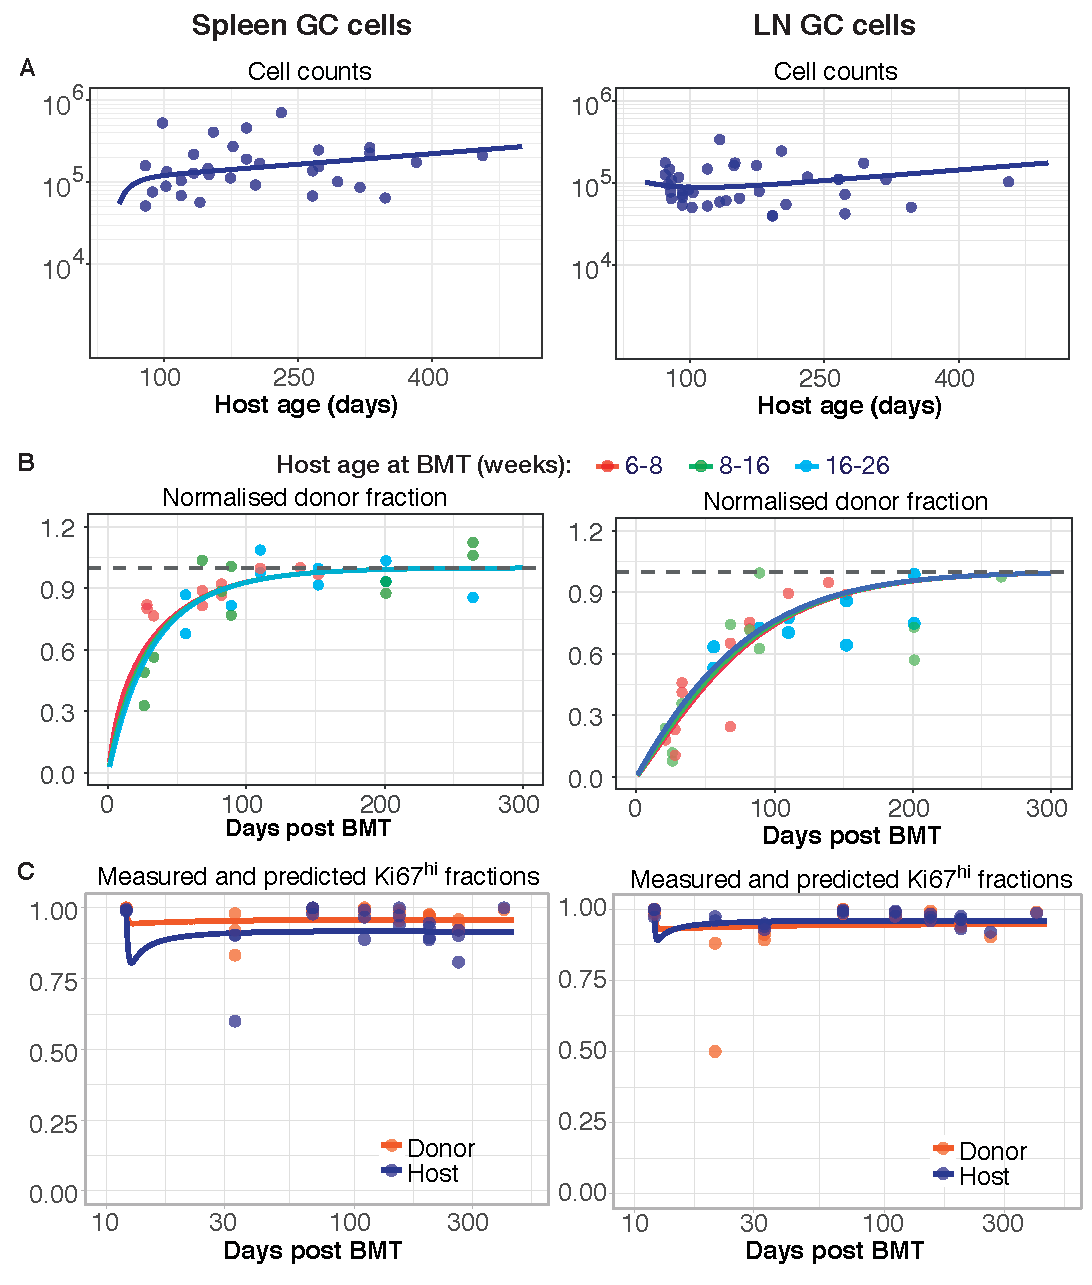
\includegraphics[scale = 0.8] {Results_GC.pdf}}
	\caption{\small \textbf{Fitted and predicted population dynamics of spleen and LN GC B cells, using the best-fitting model in which cells the net loss rate of cells remain constant with time.}  (A) The model was fitted simultaneously to the extended time-courses of total cell counts of spleen and LN GC B cells pooled in busulfan chimeras,  and their donor fractions normalised to the chimerism in FM B cells. The latter took account of different ages at BMT (right-hand panel, coloured lines; each generated using the  mode of the age within each group). (C) We then used the model parameters to predict the proportion of cells that were \khi\ within host and donor spleen and LN GC B cells over time.}
	\label{fig:results_GC}
\end{figure}



%: Table 1
\begin{table}[h!]
	\begin{center}
		\renewcommand{\arraystretch}{1.25}
		\begin{tabular}{ l c c c c} 
			\toprule 
			& \multicolumn{4}{c}{\textbf{Model and $\Delta$AIC}} \\
			\cline{2-5}
			\textbf{population}  &  {\small Simple homogeneous}  & {\small Time-dependent} &  {\small Kinetic heterogeneity} & {\small Incumbent}  \\ 
			\toprule
			Spleen GC cells     & 0      &  2  & 0 & 310  \\ 
			LN GC cells         & 2      &  5  & 0 & 250   \\ 
			\hline
			\toprule 
		\end{tabular}
	\end{center}
	\caption{\small \textbf{Comparison of AIC values for different models fitted to cell counts and donor fractions in spleen and LN GC B cells normalised to the chimerism in FM cells (spleen + LN).}} 
\label{tab:GC-AICs}
\end{table} 

%: Table 2
\begin{table}[h!]
	\begin{center}
		\renewcommand{\arraystretch}{1.25}
		\begin{tabular}{l l r l } 
			\toprule 
			\textbf{Population} & \textbf{Parameter}  &  {\small Estimate}  &  {\small 95\% CI} \\ 
			\toprule
			\textbf{Lymph node GC cells} & Total cell numbers at age 7 wks ($\times 10^{-3}$)      & 104      &  (46, 230)  \\ 
			& Total daily influx from FM into LN GC at age 7 wks ($\times 10^{-3}$)           &   1.8    &  (1.3, 2.4)  \\
			& Mean clonal life-time (days)      & 41     &  (31, 64)  \\ 
			\textbf{Splenic GC cells} & Total cell numbers at age 7 wks ($\times 10^{-3}$)      & 10.5      &  (0.15, 735)  \\ 
			& Total daily influx from FM into spleen GC at age 7 wks ($\times 10^{-3}$)           & 6.6      &  (4.7, 9.1)  \\
			& Mean clonal life-time (days)      & 15     &  (12, 21)  \\ 
			\hline
			\toprule 
		\end{tabular}
	\end{center}
	\caption{\small \textbf{Parameter estimates from the best-fit (simple homogeneous) model for spleen and LN GC B cells.}  Confidence intervals were estimated using the inverse of the Hessian matrix at the ML estimates of the parameters.}
	\label{tab:GC-parestm}
\end{table} 


\clearpage

\section*{Methods}

\section*{Predicting the kinetics of Ki67 expression in host and donor FM cells}

We divide host and donor cells into recently divided (\khi) and quiescent (\klo) compartments (Figure~\ref{fig:Ki67schematic}).

\begin{figure}[htbp]
	\centerline{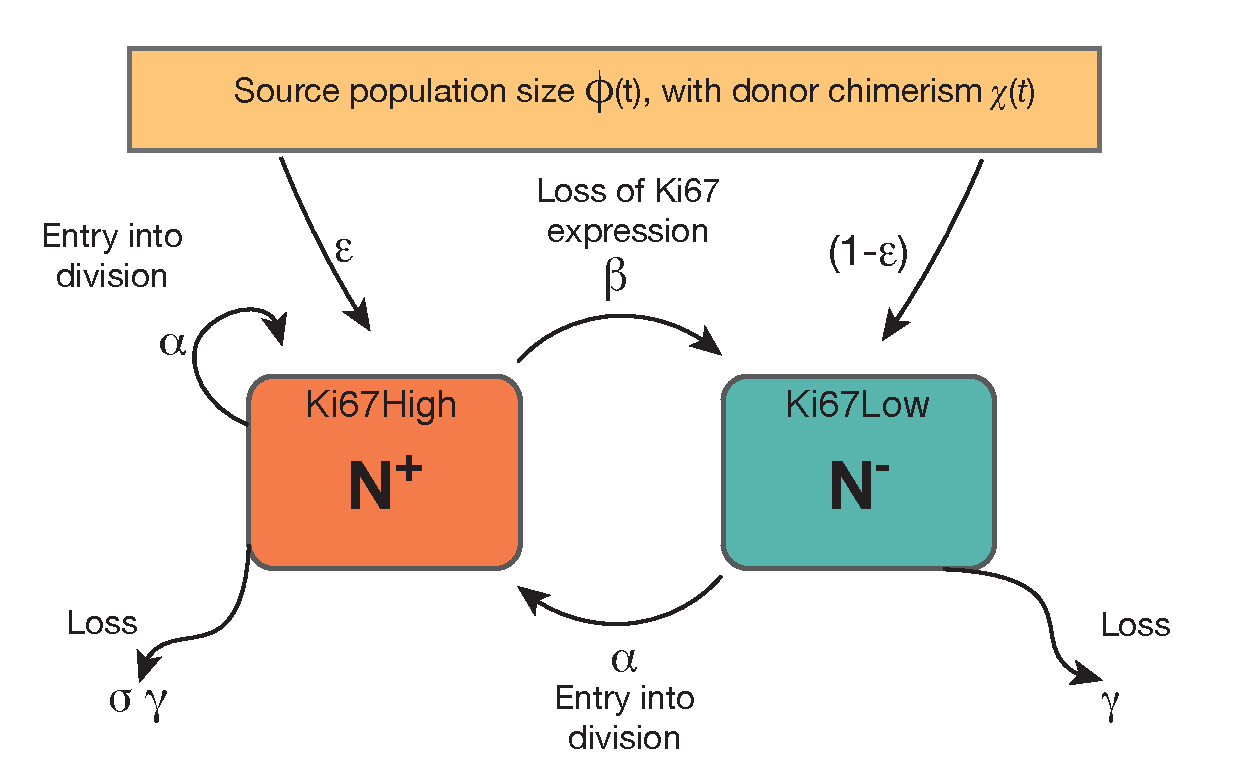
\includegraphics[scale = 0.5] {TwoComp_ki67.pdf}}
	\caption{Two compartment model for prolifeartion and loss of B cells using Ki67 as a marker for dividing and recently divided cells \label{fig:Ki67schematic}}
\end{figure}

This system is represented by the following coupled ordinary differential equations:
\begin{eqnarray}
\begin{aligned}
\frac{dN^+}{dt} &= \epsilon \, \phi(t) + \alpha \, (2\, N^- + N^+) - \beta N^+ - \sigma \, \gamma N^+ ,\\
\frac{dN^-}{dt} &=  (1-\epsilon) \, \phi(t) - \alpha N^-  + \beta N^+ - \gamma  N^+.
\end{aligned}
\label{eq:ode_ki67}
\end{eqnarray}

Here,
\begin{itemize}
\item $\epsilon$ denotes the proportion of the cells entering from source  that are \khi. Estimated from the data ($\simeq$ 0.8 for T2s and 0.1 for FMs).
%\item $\chi(t)$ is the time-varying chimerism of the source, estimated from the data and averaged over all mice.
\item $\gamma$ is the rate of loss (death + maturation) of \klo\ cells.
\item In general it is possible that recently-divided \khi\ cells may have different susceptibility to loss than quiescent (\klo) cells. The parameter $\sigma$ is the relative loss rate of \khi\ and \klo\ cells. In the simulations we ran we assumed $\sigma=1$.
\item $\alpha$ is the rate of entry into division for both \klo\ and \khi\ cells. The mean inter-division time is $1/\alpha$.
\item $\beta$ is the rate of loss of Ki67 expression after mitosis.  We and others have estimated the mean expression time $\frac{1}{\beta}$  to be 3.5 days. 
\end{itemize}

The quantities $\phi(t)$ and  $\chi(t)$, are obtained from splines fitted to the numbers of host and donor cells in the source populations.

The total size of GC population is then derived by summing up \khi and \klo subsets from equation~\ref{eq:ode_ki67}.
%Adding the equations for \khi and \klo (eq.\ref{eq:ode_ki67}) gives us the equation for the total cell counts.
\bea
\begin{aligned}
&\frac{dN}{dt} =  \phi(t) + \alpha \, N -  \gamma \, N \, ( \sigma \, \kappa + 1 - \kappa)  \\
&\frac{dN}{dt} =  \phi(t) + \alpha \, N -  \gamma \, N   \qquad \qquad \qquad \qquad \qquad \text{for} \, \sigma = 1,
\end{aligned}
\label{eq:ode_ki67_total}
\eea
where $\kappa$ is the fraction of \khi cells in the given population.

(i) For FM cells, we compare the equations~\ref{eq:FM_total} and \ref{eq:ode_ki67_total}, which shows that $\gamma = \delta_0 \, e^{-r \, t}$ and $\alpha = \rho$. We use the estimates of $\delta_0$, r and $\rho$  obtained from the fits to cell counts and normalised donor fractions.

(ii) For GC cells we calculate $\alpha$ and $\gamma$ using the estimate of net loss rate $\lambda$ obtained from the fits to the cell counts and normalised donor fractions, as described in [Hogan et al., PNAS 2015].

\red{The influx from the source population changes very slowly relative to the rates of flow between \khi\ to \klo\ and so we assume that these populations (N$^+$ and N$^-$) are in quasi-equilibrium. (This means they are locked into the kinetics of the source population and don't slosh around as the influx is changing. Think about being able to keep your balance standing on a moving train -- if it's not too jerky you can keep stably upright because the timescale over which your muscles can respond is pretty quick. If the train accelerates or decelerates fast, you will respond by lurching around a bit before you regain equilibrium)}.

We then solve the coupled ODE described in eq.~\ref{eq:ode_ki67} numerically using initial numbers of \klo\ and \khi\ host and donor cells taken from the experimental obervations at $t_{0}$ = 12 days post BMT.  We solve them twice -- once for host cells with influx $\phi(t) (1 -\chi(t))$, and again for donor cells with influx $\phi(t) \chi(t)$. We then calculate the predicted \khi\ proportions $N^{+}/(N^{+} + N^{-})$ in host and donor cells over time.

\end{document}





\textbf{Mathematical models used to describe B cell population dynamics}
\paragraph*{Constant birth-death model:}
\textit{All cells behave identically at all times.} \\
In this model we assume that cells follow random birth-death processes to form a kinetically homogeneous population that self renews through homeostatic division and decays either by death or maturation. 
Per capita net loss rate `$\lambda$' is given by loss - proliferation ($\delta - \rho$)  and is assumed to be constant over time. \\
Abbereviated as CBDM

\be
\frac{dN}{dt} = \phi[t] \, - \lambda \, N(t)
\label{eq:SHM}
\ee

\paragraph*{Time-dependent model:} 
\textit{All cells behave identically at a given instant of time.} \\
This is also a homogeneous model where all cells obey the same rules of turnover. We assume that the fitness of the whole population changes over time/host-age, due to host-intrisic factors. 
The net loss rate $\lambda$ varies with time. We explored different forms of lambda changing with time and the best-fit was obtained with the very general form representing slow exponential decline in $\lambda$ with host age, $\lambda(t) = \lambda_0 \, e^{-r\,t}$.
Abbereviated as TDM

\be
\frac{dN}{dt} = \phi[t] \, - \lambda(t) \, N(t)
\label{eq:TDM}
\ee


\paragraph*{Age-structured model:} 
\textit{This is a heterogeneous model} \\
In this model the ability of individual cells to die or divide varies with their cell-age. 
The net loss rate $\lambda$ is a function of cell's age in the current lineage. 
Changes in fitness of individual cells with age could arise as a result of adaptive changes in cell-intrisic factors and/or conditioning that cells receive through micro-environmental inteactions (host intrisic factors) throughot their lifetime.
We explored different forms of $\lambda(a)$ changing with cell age and the best-fit was obtained by, $\lambda(a) = \lambda_0 \, e^{-r \,a} $.
The PDE described in eq.~\ref{eq:ASM} tracks the population dynamics of $N(a,t)$ over time.
We also assume that the fitness of individual cells is inherited by their daughter cells.
Abbereviated as ASM

\be
\frac{\partial{N(a,t)}}{\partial{a}} + \frac{\partial{N(a,t)}}{\partial{t}} = - \lambda(a) N(a,t),
\label{eq:ASM}
\ee

We solved Equation~\ref{eq:ASM} by the method of characteristics and using two boundary conditions. One is the constraint that the population density of cells of post-thymic age $a=0$, $N(t,0)$, at any time $t$  is simply the rate of source influx at that moment, $\phi(t)$. The second boundary condition is the population density with respect to cell age at time zero, $N(0,a) = g(a)$. We can then track both (i) the fate of the population present at time zero, $N_\text{init}(t,a)$,  and (ii) the fates of cells subsequently matured from T2 cells, $N_\phi(t,a)$;
\be
\begin{aligned} 
	N_\text{init}(t,a) &= g(a-t) \exp \bigg( - \int_0^t \lambda(\tau + a - t) \, d\tau \bigg), \, \text{for} \, a \ge t \\ 
	N_phi(t,a) &= phi(t-a) \exp \bigg (- \int_0^a \lambda(\tau) \, d\tau \bigg), \, \text{for}  \, a \le t \\ 
\end{aligned} 
\label{fig:PDEsolution}
\ee 
We consider three subsets: The host population generated pre-BMT $N_\text{init}^h (t,a)$, the host population post-BMT $N_phi^h (t,a)$, and the donor population post-BMT $N_phi^d (t,a)$. We add these subsets and integrate over cell age to obtain total cell counts.
\be
N_\text{total}(t) = \int_0^t \left ( N_\text{init}^h (t,a) + N_{\phi}^h (t,a)+ N_{\phi}^d (t, a) \right ) \, da 
\ee

We used the exponential ($\lambda(a) = \lambda_0 \, e^{-a/r}$) form for the net loss rate $\lambda$ decreasing with cell age. The population density of B cells with respect to cell age at time zero is unknown and we model it as $ g(a) = \, e^{p a} \, \phi_0 $. The free parameter $p$ can be positive or negative, such that older cells can initially be over- or under-represented compared to younger cells. This definition of $g(a)$ also ensures, for consistency, that $g(0)$ is the rate of influx at t0, $\phi_{0}$.  This quantity is unknown but can be expressed in terms of $g(a)$ and the initial pool size  $N_0$;
\be
\text{Total cell numbers} = \int_0^{t_0} g(a) \, da = \int_0^{t_0} e^{p a} \, \phi_0 \, da= N_{0} \implies   \phi_0 = \frac{N_{0} p}{e^{\,p \,t_a}-1} ,
\ee 
where the range of possible cell ages at host age $t_{0}$ is $0 \le a \le t_{0}$. 

Busulfan treatment results in  levels of chimerism that vary slightly across mice. To compare replacement across mice, we normalised the  fraction of cells in the periphery that were donor-derived to the chimerism in source compartment $\chi$.
\be
\text{Normalised donor fraction} \; f_{d} = \frac{N^d_{\phi}(t)} {\chi \, N_\text{total}(t)} \\
\ee 
To incorporate data from bone marrow transfers made in recipients with different ages, we tracked the changes in the numbers of (i) the cells present at $t_0$, until the host's age at BMT ($t_b$), which were present with age distribution $g(a)$ at time $t_{0}$; and (ii) the cells matured from T2 between $t_0$ and BMT. 
\be
\begin{aligned} 
	G(a) =\,\, & \left\{ 
	\begin{aligned} 
		&g(a-(t_b-t_0)) \,\, e^{\int_{0}^{t-t_0} \lambda(\tau) d\tau} \quad \quad \qquad a \geq t_b-t_0\ \\ 
		&\phi(t_b-t_0-a) \,\, e^{\int_{0}^{a} \lambda(\tau) d\tau} \quad \,\, \quad \quad \qquad a \le t_b-t_0\ 
	\end{aligned} 
	\right\} \\ 
\end{aligned} 
\\
\ee
The cell-age distribution at BMT  is therefore a composite function $G(a)$ that tracks the cells with age distribution $g(a)$ at the age of the mice with the earliest BMT, and also those cells exported from the thymus until the age of BMT. The model can therefore accommodate differences between mice in their age at BMT. Best-fit values of the unknown parameters - $N(0)$, $p$, $\lambda_0$, and $r$ were obtained by simultaneously fitting to the log-transformed cell counts and untransformed normalised donor fractions, in {\it R} using  the Nelder-Mead algorithm.


\paragraph{Incumbent model:}
\textit{This is also a heterogeneous model} \\
 The incumbent model (Hogan et al. 2015) considers that a B cell poulation is composed of kinetically distinct subpopulations - (i) an incumbent subset of older, self-renewing cells that are resistant to displacement by new cells and (ii) a displaceble subset that turns over with a constant rate `$\lambda$' and is replaced continuously by cohorts of new cells entering the pool.
 
\be
\begin{aligned}
 &\frac{dN_{\text{donor}}}{dt} = \chi \, \phi_0 \, e^{-\nu t} - \lambda \, N_{\text{donor}}(t) \\
 &\frac{dN_{\text{host}}}{dt} = (1-\chi) \, \phi_0 \, e^{-\nu t} - \lambda \, N_{\text{host}}(t)\\
 &\frac{dI}{dt}   = -\lambda_i I(t) 
\end{aligned}
\ee
 
As described in (Hogan et al. 2015), we solved these ODEs  to obtain total cell counts $N(t)$, with initial condition $N(0) - I(0) = N_{\text{donor}}(0) + N_{\text{host}}(0)$, where $N_{\text{donor}}(0)$, $N_{\text{host}}(0)$ and $I(0)$ are the numbers of donor, host and incumbent cells present at $t_0$, respectively. We accounted for different ages at BMT,  by tracking changes in initial donor population $N_{\text{donor}}(0)$ at different recipient ages. The initial cell counts and normalised donor fraction at the given age of BMT are then
\be
\begin{aligned}
&N(t_b) = \frac{\phi(t-t_0) \, \, (e^{(\lambda - \nu) (t_b-t_0)} - 1) + (\lambda-\nu) \, (N(0)-I(0)) + (\lambda-\nu) \, \, I(0) \, e^{(\lambda - \lambda_i) (t_b-t_0)}} {(\lambda-\nu) \,\, e^{\lambda (t_b-t_0)}} \\
\\
&f_d(t_b) = \frac{N(0) \,f_d(0) \, e^{-\nu (t_b-t_0)} }{N(t_b)}
\end{aligned}
\ee
and the total cell counts and normalised donor fraction as functions of host age are
\be
\begin{aligned}
&N(t) = \frac{\phi(t-t_0) \, \, e^{-\nu(t_b-t_0)} \, \,  (e^{(\lambda - \nu) (t-t_b)} - 1) + (\lambda-\nu) \, (N(t_b)-I(t_b)) + (\lambda-\nu) \, \, I(t_b) \, e^{(\lambda - \lambda_i) (t-t_b)}} {(\lambda-\nu) \,\, e^{\lambda (t-t_b)}}\\
\\
&f_d(t) = \frac{\phi(t-t_0) \, \, e^{-\nu(t_b-t_0)} \, \, (e^{(\lambda - \nu) (t-t_b)} - 1) + (\lambda-\nu) \,  N(t_b) \, f_d(t_b)}{ \phi(t-t_0) \, \, (e^{(\lambda - \nu) (t-t_b)} - 1) + (\lambda-\nu) \, (N(t_b)-I(t_b)) + (\lambda-\nu) \,\, I(t_b) \, e^{(\lambda -\lambda_i) \, (t-t_b)}}
\end{aligned}
\ee

The incumbent model has four free parameters ($N(0)$, $\phi_0$, $I(0)$ and $\lambda$) when fitted from t0 (the age of youngest animal at BMT) since fd(0) = 0.
 
 
\clearpage

\section*{Appendix}
\section*{Modelling chimerism dynamics in the source compartment}
In order to compare the inflitartion of donor cells into the FM pool across all animals that have varying levels of chimersim in their bone marrow cell populations, we normalise the fraction of donor cells in FM pool by dividing with the value of chimerism `$\chi$' in their immediate source i.e. T2 compartment.
Therefore the quantity, normalised donor fraction $f_{d}$, is independent of chimerism and is only sensitive to parameters that are common across animals.
We describe the changes in chimerism over time using a phenomenological function (equation~\ref{eq:chimerism})  that reasonably depicts the shape of the timecourse of fraction of donor cells across all animals.

\be
\chi(t) = \chi_{stable} \, (1 - e^{-q \,t}) 
\label{eq:chimerism}
\ee

Parameters `$\chi_{stable}$' and `q' are estimated by fitting the spline in equation~\ref{eq:chimerism} to the observed donor fractions in T2 compartment.


\section*{Modelling Source influx}
We assumed that the rate of influx from source $\psi$, stays constant and used the cell counts of Transitional 2 (T2) compartment as a proxy to estimate the number of cells maturing into the FM pool.  
Equation~\ref{eq:source}, is a spline that is used to describes the changes in T2 cells over time. 
Parameters $S_0$ and $\nu$ are estimated by fitting the spline in equation~\ref{eq:source} to the observed cell counts of T2 compartment.

\be
S(t) = S_0 \, e^{-\nu \, t}
\label{eq:source}
\ee
The counts of total, donor and host T2 cells entering the FM pool at any instant is given by equation~\ref{eq:influx}. The rate constant $\psi$ is estimated using model fits to cell counts and donor fractions.
\bea
\begin{aligned}
&\phi(t) = \psi \, S(t) \\
&\phi_{\text{donor}}(t) = \psi \, S(t) \, \chi(t)   \\
&\phi_{\text{host}}(t) = \phi(t) - \phi_{\text{donor}}(t) 
\end{aligned}
\label{eq:influx}
\eea

\begin{figure}[h!]
	\centerline{\includegraphics[scale = 0.9] {Source_FM.pdf}}
	\caption{\small \textbf{Dynamics of cell counts and chimerism in the source compartment (T2 cells).}  }
	\label{fig:Source_FM}
\end{figure}





\clearpage



%: Table 1
\begin{table}[h!]
	\begin{center}
		\renewcommand{\arraystretch}{1.25}
		\begin{tabular}{ l | c c | c c | c c | c c } 
			\toprule 
			& \multicolumn{2}{c|}{\textbf{AIC}} & \multicolumn{2}{c|}{\textbf{Mean residence time}}  & \multicolumn{2}{c|}{\textbf{log(2)/r$^\ast$ estimates}}  & \multicolumn{2}{c}{\textbf{Inter-division time}} \\
			\cline{2-9}
			\textbf{Model}  &  {\small T1}  &  {\small T2} & {\small T1} & {\small T2} &  {\small T1}  &  {\small T2} & {\small T1} & {\small T2} \\ 
			\toprule
			Time-dependent            & 7.8   &  9.1 & 18(7, 44) & 17 (6, 54) & 250(46, 1300)  & 520(110, 2800) & 69(2, 2800) & 56 (3.5, 900)\\ 
			Age-structured            & 35   &  21 &  20(16, 26) & 33(21, 39) & NA  & NA &  89(36, 210) & 2000 (1300, 3300) \\ 
			\cline{4-9} 
			& \multicolumn{2}{c|}{\textbf{}} & \multicolumn{2}{c|}{\textbf{1/$\lambda_1^{\dagger}$ }}  & \multicolumn{2}{c|}{\textbf{$1/\lambda_2^{\dagger}$}} & \multicolumn{2}{c}{\textbf{}} \\
			\cline{4-9}
			constant birth-death       & 34  &  21 & 40(35, 47) & 34(30, 41) & -- & -- & -- & -- \\ 
			Incumbent                 & 34   &  21 & 39(34, 47) & 34(29, 40) & --  & -- & -- & -- \\ 
			Kinetic heterogeneity     & 34   &  21 & 41(37, 46) & 17 (6, 54) & 33(10,102) & 26(14, 47)  & -- & -- \\ 
			\hline
			\toprule 
		\end{tabular}
	\end{center}
	\caption{\small Comparison of AIC values for different models fitted to cell counts and donor fractions$^{\dagger}$ in FM B cells (Spleen + LN).}
	$^{\dagger}$ \footnotesize For the incumbent and constant birth-death model we only have $\lambda$ estimates which are quoted in 1/$\delta$ column.
	$^\ast$ \footnotesize r is the rate of change of residence-time with host-age or cell age, hence log(2)/r denotes the avearge time taken for men residence time to double. Changing $\rho$ with time or cell age gives (visually) poor fits hence not included in this analysis. \\
	\footnotesize NA - estimates for `r' are close to zero therefore log(2)/r $\sim$ NA/Inf. This shows that in this case there is very little or no effect of cell age on $\delta(a)$.
	\label{tab:FMs}
\end{table} 

\blue{Note: Age-structured model gives visually bad fits for FM cells. \\
	When  fitting FM cells with the incumbent model, size of the incumbent population is estimated to be $\approx$ 0, making it equivalent to constant birth-death model. When fitting MZ model the counts of incumbent cells are estimated $\approx 10^5$. }


%: Table 1
\begin{table}[h!]
	\begin{center}
		\renewcommand{\arraystretch}{1.25}
		\begin{tabular}{ l | c c | c c |c c |c c } 
			\toprule 
			& \multicolumn{2}{c|}{\textbf{AIC}} & \multicolumn{2}{c|}{\textbf{Mean residence time}}  & \multicolumn{2}{c|}{\textbf{log(2)/r$^\ast$ estimates}}  & \multicolumn{2}{c}{\textbf{Inter-division time}} \\
			\cline{2-9}
			\textbf{Model}  &  {\small T1}  &  {\small T2} & {\small T1} & {\small T2} &  {\small T1}  &  {\small T2} & {\small T1} & {\small T2} \\ 
			\toprule
			Time-dependent            & 32   &  66 & 19(7, 55)  & 32(11, 90) & 800(240, 2600) & 810(200,3200) & 28(7, 120) & 64(9,460) \\ 
			Age-structured            & 41   &  63 & 9(5, 16) & 11(5, 23)  & 1100(590, 2100) & 630(270, 1400) & 11(5, 22) & 15(6, 38) \\
			\cline{4-9} 
			& \multicolumn{2}{c|}{\textbf{}} & \multicolumn{2}{c|}{\textbf{1/$\lambda_1^{\dagger}$ }}  & \multicolumn{2}{c|}{\textbf{$1/\lambda_2^{\dagger}$}} & \multicolumn{2}{c}{\textbf{}} \\
			\cline{4-9}
			constant birth-death      & 44  &  68 & 111 (142, 100) & 90 (66, 125) & -- & -- & -- & -- \\ 
			Incumbent                 & 43   &  67 & 103(73, 171) & 67(45, 125) &  -- &  -- &  -- & --  \\ 
			Kinetic heterogeneity     & 40   &  66 & 270(106, 710) & 170(34, 840) & 73(52, 102) & 63(18, 210)& -- & -- \\ 
			\hline
			\toprule 
		\end{tabular}
	\end{center}
	\caption{\small Comparison of AIC values for different models fitted to cell counts and donor fractions$^{\dagger}$ in MZ B cells (Spleen).}
	$^{\dagger}$ \footnotesize For the incumbent and the constant birth-death model we only have $\lambda$ estimates which are quoted in 1/$\delta$ column. For the kinetic heterogenity model there are two subsets with different loss rates $\lambda_1$ and $\lambda_2$.
	$^\ast$ \footnotesize r is the rate of change of residence-time with host-age or cell age, hence log(2)/r denotes the avearge time taken for men residence time to double. Changing $\rho$ with time or cell age gives (visually) poor fits hence not included in this analysis. 
	\label{tab:MZs}
\end{table} 


\end{document}












